\documentclass{article}

\usepackage[a4paper, top=3cm, bottom=3cm]{geometry}
\usepackage[latin1]{inputenc}
\usepackage{setspace}
\usepackage{fancyhdr}
\usepackage{tocloft}
\usepackage{amsmath,amssymb}
\usepackage{amsbsy}
\usepackage{soul,xcolor}
\usepackage{hyperref, url}
\usepackage{caption, subcaption}
\usepackage{mathtools}
\usepackage{multirow}
\usepackage{listings}
\usepackage{algorithm, algorithmic}
\usepackage{hyperref}

\usepackage{tikz}
\tikzset{
  treenode/.style = {shape=rectangle, rounded corners,
                     draw, align=center,
                     top color=white, bottom color=blue!20},
  root/.style     = {treenode, font=\Large, bottom color=red!30},
  env/.style      = {treenode, font=\ttfamily\normalsize},
  dummy/.style    = {circle,draw}
}
\usetikzlibrary{positioning,shapes,arrows,bayesnet}


\DeclareMathOperator*{\argmax}{argmax}
\DeclareMathOperator*{\argmin}{argmin}
\newcommand{\dd}[1]{\mathrm{d}#1}
\DeclarePairedDelimiter\ceil{\lceil}{\rceil}
\DeclarePairedDelimiter\floor{\lfloor}{\rfloor}

\newcommand{\vect}[1]{\overrightarrow{#1}}

\newcommand\Myperm[2][^n]{\prescript{#1\mkern-2.5mu}{}P_{#2}}
\newcommand\Mycomb[2][^n]{\prescript{#1\mkern-0.5mu}{}C_{#2}}

%\DeclarePairedDelimiter{\norm}{\lVert}{\rVert}
\newcommand{\norm}[1]{\left\lVert#1\right\rVert}


\title{Tree}
\author{Jyotirmoy Banerjee}
\begin{document}
\maketitle


\section{Decision tree}
Decision Trees are an important type of algorithm for predictive modelling machine learning.
The classical decision tree algorithms have been around for decades and modern variations like random forest are among the most powerful techniques available.
Decision tree algorithm is also known by it's more modern name CART which stands for Classification And Regression Trees. The representation for the CART model is a binary tree. Each root node represents a single input variable (x) and a split point on that variable (assuming the variable is numeric). The leaf nodes of the tree contain an output variable (y) which is used to make a prediction.

For example, given a dataset with two inputs (x) of height in centimetres and weight in kilograms the output of sex as male or female, is an example of a binary decision tree, see Figure~\ref{fig:decisiontree}.
\begin{figure}
\centering
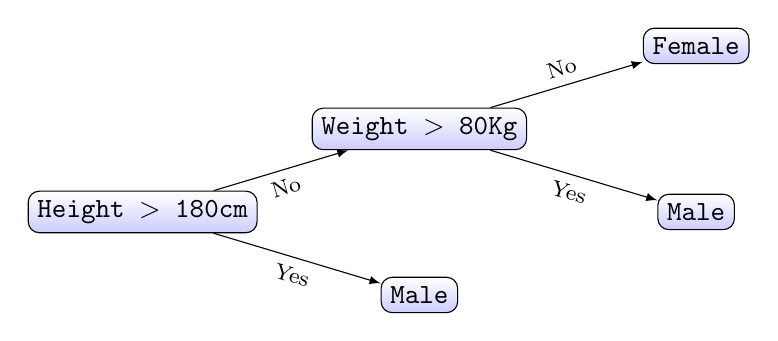
\begin{tikzpicture}
  [
    grow                    = right,
    sibling distance        = 6em,
    level distance          = 10em,
    edge from parent/.style = {draw, -latex},
    every node/.style       = {font=\footnotesize},
    sloped
  ]
  %\node [root] {Height $>$ 180}
  \node [env] {Height $>$ 180cm}
  		child { node [env] {Male}
      		edge from parent node [below] {Yes} }  
      	child { node [env] {Weight $>$ 80Kg}
      		  	child { node [env] {Male}
      				edge from parent node [below] {Yes} }   
      		  	child { node [env] {Female}
      				edge from parent node [above] {No} }        				
      		edge from parent node [below] {No} };
\end{tikzpicture}
\caption{Decision tree}
\label{fig:decisiontree}
\end{figure}
A learned binary tree is actually a partitioning of the input space. You can think of each input variable as a dimension on a p-dimensional space. The decision tree split this up into rectangles (when p=2 input variables) or some kind of hyper-rectangles with more inputs.
New data is filtered through the tree and lands in one of the rectangles and the output value for that rectangle is the prediction made by the model. This gives you some feeling for the type of decisions that a CART model is capable of making, e.g.\ boxy decision boundaries.


The selection of which input variable to use and the specific split or cut-point is chosen using a greedy algorithm to minimize a cost function. Tree construction ends using a predefined stopping criterion, such as a minimum number of training instances assigned to each leaf node of the tree.


\subsection{Greedy splitting}
Creating a binary decision tree is actually a process of dividing up the input space. A greedy approach is used to divide the space called recursive binary splitting. This is a numerical procedure where all the values are lined up and different split points are tried and tested using a cost function. The split with the best cost (lowest cost because we minimize cost) is selected. All input variables and all possible split points are evaluated and chosen in a greedy manner (e.g. the very best split point is chosen each time).

For regression predictive modelling problems the cost function that is minimized to choose split points is the sum squared error across all training samples that fall within the rectangle:
\begin{equation*}
\sum(y-\mbox{prediction})^2
\end{equation*}
where $y$ is the output for the training sample and prediction is the predicted output for the rectangle.

For classification the cost function provides an indication of how ``pure" the leaf nodes are (how mixed the training data assigned to each node is). There are three commonly used impurity measures used in binary decision trees: Entropy, Gini index, and Classification Error.
\begin{align*}
\mbox{Entropy} &= - \sum_j p_j \log p_j \\
\mbox{Gini} &= 1 - \sum_j {p_j}^2 \\
\mbox{Classification Error} &= 1 - \max {p_j}
\end{align*}
where $p_j$ is the probability of class $j$.
The entropy is $0$ if all samples of a node belong to the same class, and the entropy is maximal if we have a uniform class distribution. In other words, the entropy of a node (consist of single class) is zero because the probability is $1$ and $\log (1) = 0$. Entropy reaches maximum value (i.e.\ 1) when all classes in the node have equal probability. Similar to entropy, the Gini index is maximal (i.e.\ 0.5) if the classes are perfectly mixed, for example, in a binary class.

We start at the tree root and split the data on the feature that results in the largest information gain. The Information Gain (IG) can be defined as follows:
\begin{equation*}
{IG}(D_p) = I(D_p) - \frac{N_{l}}{N_p}I(D_{l}) - \frac{N_{r}}{N_p}I(D_{r})
\end{equation*}
where $I$ could be entropy, Gini index, or classification error, $D_p$, $D_l$, and $D_r$ are the dataset of the parent, left and right child node.

%\href{http://www.bogotobogo.com/python/scikit-learn/scikt_machine_learning_Decision_Tree_Learning_Informatioin_Gain_IG_Impurity_Entropy_Gini_Classification_Error.php}{Example}

\begin{figure}
\centering
\begin{subfigure}{.4\textwidth}
\centering
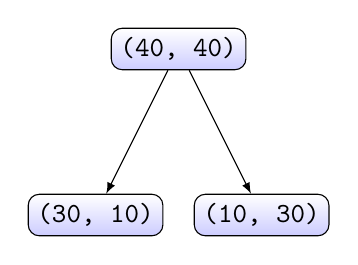
\begin{tikzpicture}
  [
    grow                    = down,
    sibling distance        = 6em,
    level distance          = 6em,
    edge from parent/.style = {draw, -latex},
    every node/.style       = {font=\footnotesize},
    sloped
  ]
  \node [env] {(40, 40)}
  		child { node [env] {(30, 10)}
      		edge from parent node [above] {} }  
      	child { node [env] {(10, 30)}      				
      		edge from parent node [below] {} };
%   \label{fig:informationgain1}
\end{tikzpicture}
\caption*{A}
\end{subfigure}
\qquad
\begin{subfigure}{.4\textwidth}
\centering
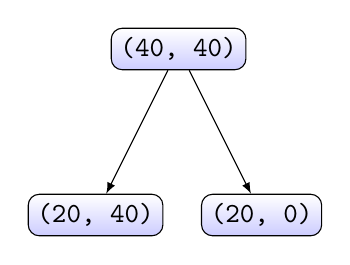
\begin{tikzpicture}
  [
    grow                    = down,
    sibling distance        = 6em,
    level distance          = 6em,
    edge from parent/.style = {draw, -latex},
    every node/.style       = {font=\footnotesize},
    sloped
  ]
  \node [env] {(40, 40)}
  		child { node [env] {(20, 40)}
      		edge from parent node [above] {} }  
      	child { node [env] {(20, 0)}      				
      		edge from parent node [below] {} };
%   \label{fig:informationgain2}
\end{tikzpicture}
\caption*{B}
\end{subfigure}
\caption{Information Gain - Example}
\label{fig:informationgain}
\end{figure}

As per the Information gain example in Figure~\ref{fig:informationgain} -
\begin{align*}
\mbox{Classification Error} &= 1 - \max p_j \\
A: I_E(D_p) &= 1 - \frac{40}{80} = 0.5\\
A: I_E(D_l)  &= 1 - \frac{30}{40} = 0.25\\
A: I_E(D_r)  &= 1 - \frac{30}{40} = 0.25\\
IG_{E} &= 0.5 - \frac{40}{80} * 0.25 - \frac{40}{80} * 0.25 = 0.25 \\
B: I_E(D_l)  &= 1 - \frac{40}{60} = \frac{1}{3}\\
B: I_E(D_r)  &= 1 - \frac{20}{20} = 0\\
IG_{E} &= 0.5 - \frac{60}{80} * \frac{1}{3} - \frac{20}{80} * 0 = 0.25 \\
\end{align*}
The information gains using the classification error as a splitting criterion are the same (0.25) in both cases A and B.
\begin{align*}
\mbox{Gini index} &= 1 - \sum_j {p_j}^2 \\
A: I_E(D_p) &= 1 - \bigg(\Big(\frac{40}{80}\Big)^2 + \Big(\frac{40}{80}\Big)^2\bigg) = 0.5\\
A: I_E(D_l)  &= 1 - \bigg(\Big(\frac{30}{40}\Big)^2 + \Big(\frac{10}{40}\Big)^2\bigg) = 0.375\\
A: I_E(D_r)  &= 1 - \bigg(\Big(\frac{10}{40}\Big)^2 + \Big(\frac{30}{40}\Big)^2\bigg) = 0.375\\
IG_{G} &= 0.5 - \frac{40}{80} * 0.25 - \frac{40}{80} * 0.25 = 0.25 \\
B: I_E(D_l)  &= 1 - \bigg(\Big(\frac{20}{60}\Big)^2 + \Big(\frac{40}{60}\Big)^2\bigg) = 0.44\\
B: I_E(D_r)  &= 1 - \bigg(\Big(\frac{20}{20}\Big)^2 + \Big(\frac{0}{20}\Big)^2\bigg) = 0\\
IG_{G} &= 0.5 - \frac{60}{80} * 0.44 - \frac{20}{80} * 0 = 0.17 \\
\end{align*}
The information gains using the Gini index favors the split B.
\begin{align*}
\mbox{Entropy} &= - \sum_j p_j \log p_j\\
A: I_E(D_p) &= - \bigg(\Big(\frac{40}{80}\Big) \log \Big(\frac{40}{80}\Big) + \Big(\frac{40}{80}\Big) \log \Big(\frac{40}{80}\Big)\bigg) = 1\\
A: I_E(D_l)  &= - \bigg(\Big(\frac{30}{40}\Big) \log \Big(\frac{30}{40}\Big) + \Big(\frac{10}{40}\Big) \log \Big(\frac{10}{40}\Big)\bigg) = 0.81\\
A: I_E(D_r)  &= - \bigg(\Big(\frac{10}{40}\Big) \log \Big(\frac{10}{40}\Big) + \Big(\frac{30}{40}\Big) \log \Big(\frac{30}{40}\Big)\bigg) = 0.81\\
IG_{H} &= 0.5 - \frac{40}{80} * 0.25 - \frac{40}{80} * 0.25 = 0.25 \\
B: I_E(D_l)  &= - \bigg(\Big(\frac{20}{60}\Big) \log \Big(\frac{20}{60}\Big) + \Big(\frac{40}{60}\Big) \log \Big(\frac{40}{60}\Big)\bigg) = 0.92\\
B: I_E(D_r)  &= - \bigg(\Big(\frac{20}{20}\Big) \log \Big(\frac{20}{20}\Big) + \Big(\frac{0}{20}\Big) \log \Big(\frac{0}{20}\Big)\bigg) = 0\\
IG_{H} &= 1 - \frac{60}{80} * 0.92 - \frac{20}{80} * 0 = 0.31 \\
\end{align*}
The information gains using the entropy criterion favors B.

%For classification the \emph{Gini} index function is used which provides an indication of how ``pure" the leaf nodes are (how mixed the training data assigned to each node is).
%\begin{equation*}
%G = \sum(p_k(1-p_k))
%\end{equation*}
%where $G$ is the Gini index over all classes, $p_k$ are the proportion of training instances with class $k$ in the rectangle of interest. A node that has all classes of the same type (perfect class purity) will have $G=0$, where as a $G$ that has a $50-50$ split of classes for a binary classification problem (worst purity) will have a $G=0.5$.

\subsection{Stopping criterion}
The recursive binary splitting procedure described above needs to know when to stop splitting as it works its way down the tree with the training data.
The most common stopping procedure is to use a minimum count on the number of training instances assigned to each leaf node. If the count is less than some minimum then the split is not accepted and the node is taken as a final leaf node.

The count of training members is tuned to the dataset, e.g.\ 5 or 10. It defines how specific to the training data the tree will be. Too specific (e.g.\ a count of 1) and the tree will overfit the training data and likely have poor performance on the test set.

\subsection{Pruning the tree}
The stopping criterion is important as it strongly influences the performance of your tree. You can use pruning after learning your tree to further lift performance.
The complexity of a decision tree is defined as the number of splits in the tree. Simpler trees are preferred. They are easy to understand (you can print them out and show them to subject matter experts), and they are less likely to overfit your data.

The fastest and simplest pruning method is to work through each leaf node in the tree and evaluate the effect of removing it using a hold-out test set. Leaf nodes are removed only if it results in a drop in the overall cost function on the entire test set. You stop removing nodes when no further improvements can be made.

More sophisticated pruning methods can be used such as cost complexity pruning (also called weakest link pruning) where a learning parameter (alpha) is used to weigh whether nodes can be removed based on the size of the sub-tree.

\section{Bootstrapping}
In machine learning, the \emph{bootstrap} method refers to random sampling with replacement. This sample is referred to as a resample. 
This allows the model or algorithm to get a better understanding of the various biases, variances and features that exist in the resample. Taking a sample of the data allows the resample to contain different characteristics than it might have contained as a whole.

The reason to use the bootstrap method is because it can test the stability of a solution. By using multiple sample data sets and then testing multiple models, it can increase robustness. Perhaps one sample data set has a larger mean than another, or a different standard deviation. This might break a model that was overfit, and not tested using data sets with different variations. Bootstrapping is used in both Bagging and Boosting.

\section{Bagging}
Bagging refers to bootstrap aggregation. Bagging predictors is a method for generating multiple versions of a predictor and using these to get an aggregated predictor.
What Bagging does is help reduce variance from models that are might be very accurate, but only on the data they were trained on. This is also known as overfitting. Overfitting is when a function fits the data too well. Typically this is because the actual equation is much too complicated to take into account each data point and outlier. For example, decision tree like CART has high variance.
Bagging gets around this by creating it's own variance amongst the data by sampling and replacing data while it tests multiple hypothesis (models). In turn, this reduces the noise by utilizing multiple samples that would most likely be made up of data with various attributes (median, average, etc).

Once each model has developed a hypothesis. The models use voting for classification or averaging for regression. This is where the `Aggregating' in `Bootstrap Aggregating' comes into play. Each hypothesis has the same weight as all the others. When we later discuss boosting, this is one of the places the two methodologies differ.
Essentially, all these models run at the same time, and vote on which hypothesis is the most accurate. This helps to decrease variance i.e.\ reduce the overfit.
Bagging is the application of the Bootstrap procedure to a high-variance machine learning algorithm, typically decision trees.

Let's assume we have a sample dataset of 1000 instances and we are using the CART algorithm. Bagging of the CART algorithm would work as follows:
\begin{enumerate} \addtolength{\itemsep}{-0.5\baselineskip}
\item Create many (e.g. 100) random sub-samples of our dataset with replacement.
\item Train a CART model on each sample.
\item Given a new dataset, calculate the average prediction from each model.
\end{enumerate}
For example, if we had 5 bagged decision trees that made the following class predictions for a in input sample: blue, blue, red, blue and red, we would take the most frequent class and predict blue.

When bagging with decision trees, we are less concerned about individual trees overfitting the training data. For this reason and for efficiency, the individual decision trees are grown deep (e.g. few training samples at each leaf-node of the tree) and the trees are not pruned. These trees will have both high variance and low bias. These are important characterize of sub-models when combining predictions using bagging.

The only parameters when bagging decision trees is the number of samples and hence the number of trees to include. This can be chosen by increasing the number of trees on run after run until the accuracy begins to stop showing improvement (e.g.\ on a cross validation test harness). Very large numbers of models may take a long time to prepare, but will not overfit the training data.
Just like the decision trees themselves, Bagging can be used for classification and regression problems.

\subsection{Random forest}
Random Forests are an improvement over bagged decision trees. A problem with decision trees like CART is that they are greedy. They choose which variable to split on using a greedy algorithm that minimizes error. As such, even with Bagging, the decision trees can have a lot of structural similarities and in turn have high correlation in their predictions.

Combining predictions from multiple models in ensembles works better if the predictions from the sub-models are uncorrelated or at best weakly correlated. Random forest changes the algorithm for the way that the sub-trees are learned so that the resulting predictions from all of the sub-trees have less correlation.

It is a simple tweak. In CART, when selecting a split point, the learning algorithm is allowed to look through all variables and all variable values in order to select the most optimal split-point. The random forest algorithm changes this procedure so that the learning algorithm is limited to a random sample of features of which to search.

The number of features that can be searched at each split point ($m$) must be specified as a parameter to the algorithm. You can try different values and tune it using cross validation.
\begin{enumerate} \addtolength{\itemsep}{-0.5\baselineskip}
\item For classification a good default is: $m = \sqrt{p}$
\item For regression a good default is: $m = p/3$
\end{enumerate}
where m is the number of randomly selected features that can be searched at a split point and p is the number of input variables. For example, if a dataset had 25 input variables for a classification problem, then:
\begin{enumerate} \addtolength{\itemsep}{-0.5\baselineskip}
\item $m = \sqrt{25}$
\item $m = 5$
\end{enumerate}

\subsubsection{Hyperparameters}
In the case of a random forest, hyperparameters include:
\begin{enumerate}
\item \texttt{n\_estimators} = number of trees in the foreset
\item \texttt{max\_features} = max number of features considered for splitting a node
\item \texttt{max\_depth} = max number of levels in each decision tree
\item \texttt{min\_samples\_split} = min number of data points placed in a node before the node is split
\item \texttt{min\_samples\_leaf} = min number of data points allowed in a leaf node
\item \texttt{bootstrap} = method for sampling data points (with or without replacement)
\end{enumerate}

\section{Boosting}
Boosting refers to a group of algorithms that utilize weighted averages to make weak learners into stronger learners. Unlike bagging that had each model run independently and then aggregate the outputs at the end without preference to any model. Boosting is all about `teamwork'. Each model that runs, dictates what features the next model will focus on.
Boosting also requires bootstrapping. However, there is another difference here. Unlike in bagging, boosting weights each sample of data. This means some samples will be run more often than others.

When boosting runs each model, it tracks which data samples are the most successful and which are not. The data sets with the most misclassified outputs are given heavier weights. These are considered to be data that have more complexity and requires more iterations to properly train the model.
During the actual classification stage, there is also a difference in how boosting treats the models. In boosting, the model's error rates are kept track of because better models are given better weights.
That way, when the `voting' occurs, unlike in bagging, the models with better outcomes have a stronger pull on the final output.

Boosting and bagging are both great techniques to decrease variance. Ensemble methods generally out perform a single model. There are different reasons you would use one over the other. Bagging is great for decreasing variance when a model is overfit. However, boosting is much more likely to be a better pick of the two methods. Boosting also is much more likely to cause performance issues. It is also great for decreasing bias in an underfit model. 


Boosting algorithms, such as AdaBoost, are iterative algorithms that place different weights on the training distribution each iteration. After each iteration boosting increases the weights associated with the incorrectly classified examples and decreases the weights associated with the correctly classified examples. This forces the learner to focus more on the incorrectly classified examples in the next iteration. Because rare classes/cases~\cite{DBLP:journals/sigkdd/Weiss04} are more error-prone than common classes/cases, it is reasonable to believe that boosting may improve their classification performance because, overall, it will increase the weights of the examples associated with these rare cases/classes. Note that because boosting effectively alters the distribution of the training data, one could consider it a type of advanced sampling technique.

\subsection{Additive model}
These models are fit by minimizing a loss function averaged over the training data, such as squared-error or a likelihood-based loss function,
\begin{align*}
\min_{\{\beta_m,\gamma_m\}} \sum_{i=1}^{N} L(y_i, f(x_i)) & \\
\mbox{where} \quad f(x) &= \sum_{m=1}^{M} \beta_m \, b(x;\gamma_m)
\end{align*}
where $\beta_m, m=1,2,\cdots,M$ are the expansion coefficients, and $b(x;\gamma) \in \mathbb{R}$ are usually simple functions of the multivariate argument $x$, characterized  by a set of parameters $\gamma$.  

The above function requires computationally intensive numerical optimization techniques. A simple alternative is to solve the subproblem of fitting just a single basis at a time. This is described in the algorithm called  \emph{forward stage-wise additive modelling}.
\begin{algorithm}[h]
\caption{Forward stage-wise additive modelling}
\begin{enumerate}
\item Initialize $f_0(x) = 0$.
\item For $m = 1$ to $M$:
	\begin{enumerate}
	\item Compute
		\begin{align*}
		(\beta_m,\gamma_m) &= \argmin_{\beta,\gamma} \sum_{i=1}^{N} L(y_i, f_{m-1}(x_i) + \beta \, b(x_i;\gamma))
		\end{align*}
	\item Set $f_m(x) = f_{m-1}(x) + \beta_m \, b(x;\gamma_m)$
	\end{enumerate}
\end{enumerate}
\end{algorithm}

\subsection{AdaBoost}
AdaBoost is equivalent to forward stage-wise additive modelling using the loss function:
\begin{align*}
L(y, f(x)) &= \exp{(-y f(x))} \\
\end{align*}

In adaboost each classifier has different weights assigned to it based on the classifier's performance (more weight is assigned to the classifier when accuracy is more and vice-verse), weights are also assigned to the observations at the end of every round, in such a way that wrongly predicted observations have increased weight resulting in their probability of being picked more often in the next classifier's sample. So, the consecutive training set depends on their previous training set, and hence correlation exists between the built trees.

Thus, Adaboost increases the predictive accuracy by assigning weights to both observations at end of every tree and weights(scores) to every classifier. Hence, in Adaboost, every classifier has a different weightage on final prediction contrary to the random forest where all trees are assigned equal weights.



\subsection{Gradient Boosting Machine (GBM)}

Just like AdaBoost, Gradient Boost also combines a number of weak learners to form a strong learner. Here, the residual of the current classifier becomes the input for the next consecutive classifier on which the trees are built, and hence it is an additive model. The residuals are captured in a step-by-step manner by the classifiers, in order to capture the maximum variance within the data, this is done by introducing the learning rate to the classifiers.

By this method, we are slowly inching in the right direction towards better prediction (This is done by identifying negative gradient and moving in the opposite direction to reduce the loss, hence it is called Gradient Boosting in line with Gradient Descent where similar logic is employed). Thus, by number of classifiers, we arrive at a predictive value very close to the observed value.

Initially, a tree with a single node is built which predicts the aggregated value of $Y$ in case of regression or log(odds) of $Y$ for classification problems after which trees with greater depth are grown on previous classifier's residuals. Learning rates are given as constant for every tree so that the model takes small steps in the right direction to capture the variance and train the classifier on it. Unlike Adaboost, here all the trees are given equal weights.


\begin{table}[hbt]
\begin{tabular}{p{0.05\linewidth} | p{0.4\linewidth} | p{0.4\linewidth}}
\hline
SNo & Adaboost & Gradient Boost \\
\hline
1&  An additive model where shortcomings of previous models are identified by high-weight data points. &  An additive model where shortcomings of previous models are identified by the gradient.  \\
 2&  The trees are usually grown as decision stumps. &  The trees are grown to a greater depth usually ranging from 8 to 32 terminal nodes.  \\
 3&  Each classifier has different weights assigned to the final prediction based on its performance. &   All classifiers are weighed equally and their predictive capacity is restricted with learning rate to increase accuracy. \\
 4&  It gives weights to both classifiers and observations thus capturing maximum variance within data. &  It builds trees on previous classifier's residuals thus capturing variance in data.  \\
 \hline   
\end{tabular}
\end{table}


\end{document}

